\documentclass[18pt]{article}
\usepackage[a4paper, margin=4.cm]{geometry}
\usepackage{graphicx} % Required for inserting images

\title{CSE 300: Online Assignment}
\author{Md Shamsuzzoha Bayzid, Mahjabin Nahar, Md Shariful Islam Bhuyan \and and Md Saidur Rahman }
\date{June 2021}

\usepackage{multicol}
\usepackage{multirow}

\begin{document}

\maketitle

\section{Introduction}
This assignment has been designed to assess the preparation of the students in writing scientific articles using \LaTeX. This assignment covers a variety of components that are commonly used in scientific manuscripts.

\subsection{Equations}
Let $a_0$, $a_n$ and $b_n$ are terms of a series. Their definitions are given by Eqn. 1\\

$a_0 = \frac{1}{\pi} \int_{-\pi}^{\pi} f(x)\,dx$\\

$a_n = \frac{1}{\pi} \int_{-\pi}^{\pi} cos\,nx\,dx = \frac{1}{\pi} \int_{-\pi}^{\pi} x^2 cos\,nx\,dx$\\

$b_n = \frac{1}{\pi} \int_{-\pi}^{\pi} sin\,nx\,dx = \frac{1}{\pi} \int_{-\pi}^{\pi} x^2 sin\,nx\,dx$ \\

\noindent (1)

\subsection{Tables}
We wish to place the Table at the bottom of the page.
\begin{table}[b]
\begin{tabular}{| l || l | l | l |}
    \hline
    \multicolumn{4}{|c|}{Item List}   \\
    \hline
    Item Name or & ALPHA 2 Code & ALPHA 3 Code & Numeric Code \\
    Product Name &&&\\
    \hline
    Item001 & AF & AFG & \multirow{4}{*}{\begin{tabular}{|c|c|c|}
        \cline{1-1}
        004 & \multicolumn{2}{c}{} \\
        \cline{1-1}
        \cline{1-1}
        008 & \multicolumn{2}{c}{}\\
        \cline{1-1}
        \cline{1-1}
        009 & \multicolumn{2}{c}{}\\
        \cline{1-1}
        \hline
        012 & 013 & 014 \\
        \hline 
    \end{tabular}} \\
    Item002 & AX & ALA & \\
    Item003 & AL & ALB & \\
    Item004 & DZ & DZA & \\
    \hline
    \hline
    Item005 & AS & ASM & \multirow{3}{*}{\begin{tabular}{|c|c|c}
        \cline{1-1}
        016 & \multicolumn{2}{c}{} \\
        \cline{1-1}
        \cline{1-2}
        010 & 020 & \\
        \cline{1-2}
        \cline{1-2}
        024 & 025 & \\
        \cline{1-2}
    \end{tabular}} \\
    Item006 & AD & AND & \\
    Item007 & AO & AGO & \\
    \hline
    \hline
    \hline
    \end{tabular}
\end{table}

\subsection{Figures}
We intend to put Figure 1 at the top of a page.
\begin{figure}[t]
    \centering
    \begin{tabular}{cc}
        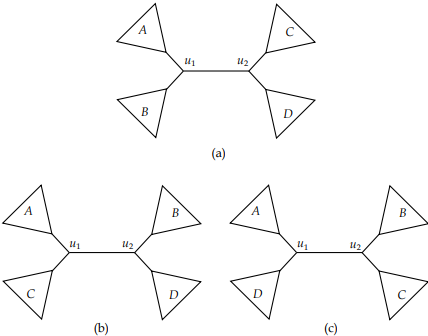
\includegraphics[angle=90]{Screenshot 2024-01-30 014001.png} & 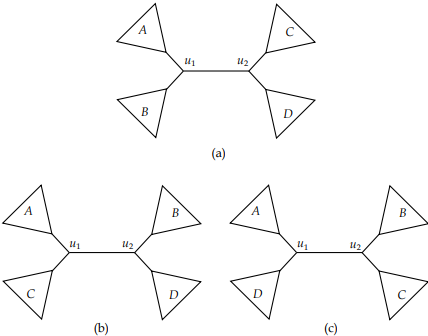
\includegraphics[angle=90]{Screenshot 2024-01-30 014001.png} \
    \end{tabular}
    \caption{Side by side same figure}
    \label{fig:enter-label}
\end{figure}

\section{Conclusions}
The major objectives of this assignment are listed below (please do not ignore the font sizes).

\begin{itemize}
    \item \Large{To assess the ability of the students in preparing manuscripts in \LaTeX.}
    \item  To see if the students have adequately practiced different aspects of writing in \LaTeX.
    \item To see if the students can add various basic components (e.g., tables, figures, equations) to a LATEX manuscript.
    \item To see if the students can leverage the available materials (both offline and online) to do something which has not explicitly been taught in the class.
    \end{itemize}
    
\end{document}
